\documentclass[12pt]{extreport}

\usepackage[a4paper, total={6in, 8in}]{geometry}
\usepackage{amsfonts}
\usepackage{amsmath}
\usepackage{amsthm}
\usepackage{hyperref}
\usepackage{tikz}
\usepackage{graphicx}
\usepackage{float}
\usepackage[utf8]{inputenc}
\usepackage{fontenc}
\usepackage[boxruled,linesnumbered]{algorithm2e}
\usepackage{booktabs}
\usepackage{multirow}
\usepackage{adjustbox}
\usepackage{cleveref}

\usepackage[sorting=none, backend=biber]{biblatex}
\usepackage{svg}

%Bibliographies
\bibliography{references,rfc}

\theoremstyle{plain}
\newtheorem{theorem}{Theorem}[section]
\newtheorem{lemma}[theorem]{Lemma}
\newtheorem{proposition}[theorem]{Proposition}
\newtheorem*{corollary}{Corollary}

\theoremstyle{definition}
\newtheorem{definition}{Definition}[section]
\newtheorem{conjecture}{Conjecture}[section]
\newtheorem{example}{Example}[section]

\theoremstyle{remark}
\newtheorem*{remark}{Remark}
\newtheorem*{note}{Note}

\crefname{algocf}{alg.}{algs.}
\Crefname{algocf}{Algorithm}{Algorithms}

%Title
\title{Some Security Considerations over Contiki-based Sensor Network}
%Authors
\author{Yan Yan}
\date{\today}

\begin{document}

\maketitle

\tableofcontents

%Body
%

\section{Introduction}

Hello, world!

\section{Introduction}
Applications for IoT flourish, leaving a great desire for not only energy efficient, cheap devices, but also for devices that support basic cryptographic functionality such as confidentiality and/or authenticity. Popular algorithms are e.g. the Advanced Encryption Standard\cite{AES} (AES) for confidentiality, and the Elliptic Curve Digital Signature Algorithm\cite{ECDSA} (ECDSA) for authenticity, which, when used in conjunction, enable applications to establish secure end-to-end channels via e.g. Datagram TLS\cite{DTLS} (DTLS). 

However whilst AES is a secure block cipher, one might require randomness to turn it into a secure encryption scheme for arbitrary length messages. Somewhat similarly, ECDSA relies on a known-to-be-secure mathematical problem. However, it also requires large and securely generated random numbers. Consequently, when supporting cryptography the secure generation of random numbers is crucial. 

%The prospering IoT applications constantly proposes higher requirements to security where cryptography plays an important role. Among all prerequisite of implementing cryptographic primitives on these IoT devices, a reliable Random Number Generator (RNG) is critical as it is required in most cryptographic algorithms. In practice, a RNG typically involves a Pseudo Random Number Generator (PRNG) seeded by a high entropy physical source.

In 2013, Texas Instruments (TI) launched a new System-on-chip (SoC), the CC2538\cite{CC2538}, featuring secure channels over 802.15.4 via multiple cryptographic hardware accelerators. Partially because of these cryptographic accelerators, projects such as Contiki\cite{Contiki} and OpenWSN\cite{OpenWSN} began to support the CC2538 with enthusiasm. As of writing this paper, the chip features in the suggested list for Zigbee and 6LoWPAN solutions on TI's website\cite{ZigbeeProducts}.

However, despite all the cryptographic hardware support, the CC2538 does not have a Random Number Generator (RNG) dedicated for cryptographic applications; instead, the user's guide suggests to use a 16 bit Linear Feedback Shift Register (LFSR) as a Pseudo RNG (PRNG) where the seed is generated by the Radio Frequency (RF) module sampling from the radio noise. Whilst the user guide at no point suggested that this method should be used in conjunction with cryptographic algorithms, developers have little choice in the absence of alternatives. Also, in the absence of published attacks, there is often a temptation to ignore warnings towards insecure RNG implementations such as in \cite{SmartMeterBlog}. 

\subsection{Our Contribution}
We show in this study that this choice proves catastrophic for cryptographic applications, not only because the in-built PRNG has only 16 bit entropy which can be easily predicted, but also because we are able to practically demonstrate how to bias the seed obtained from the RF module through the RF interface. Consequently, even if the weak in-built PRNG was replaced by a stronger component, the source for the seed could still be tampered with and thus render the system insecure. All the experimental work in this paper are performed on the latest Contiki release version 3.0.
%The related source code can be accessed at \cite{prngtest}.

Our paper is structured as follows. We begin in \Cref{ContikiDriverIssue} with some Contiki RNG driver issues for CC2538. \Cref{LFSR} revises why using a 16 bit LFSR as PRNG is a bad practice and we show how this design flaw can be exploited to break DTLS in \Cref{BreakDTLS}, before reviewing the problem in \Cref{PRNGReflection}. In \Cref{Seed} we explain how CC2538 samples the radio noise into random seed and then we demonstrate a bias attack in \Cref{Jamming} which could be achieved given physical access to the device. Finally we conclude the paper in \Cref{Conclusion}.

\subsection{Related Work}
The design flaw of using a 16 bit LFSR as PRNG has been reported by \cite{SmartMeterBlog}\cite{CC2530PRNG} on CC2430\cite{CC2430Manual} and CC2530\cite{CC2530Manual} respectively. These chips are the predecessors of CC2538 in the SimpleLink\texttrademark  series and they all adopted the same RNG design. The blogs reported the flaw and warned that it could easily be exploited to compromise the Z-Stack library\cite{ZStack} and Smart Energy Profile ECC in many Smart Meter applications. We essentially `rediscovered' that this poor design choice still features in the CC2538 product. However, whilst in previous work the possibility of injecting a jamming signal was contemplated, we are the first to actually examine the technical feasibility of this and to demonstrate a working attack.

\subsection{Contiki Driver Issues}\label{ContikiDriverIssue}
We made extensive use of Contiki in our research and fixed (and reported) some coding issues in the CC2538 RNG driver (Contiki release-3.0). These were, the reading out of the LFSR without ready check, a lack of validity check when reading random seed bits from the RF module, and a bug that drops the Most Significant Bit (MSB) and leaves the Least Significant Bit (LSB) to be constantly zero in the seed.  We modified the code and fixed these issues in our experiments. 

Another issue in the driver is that the CC2538 User's Guide\cite{CC2538Manual} suggests only to use the lower byte (8 bits) as a random number but the driver actually used 16 bits in the LFSR. However, this coding mistake does not affect our result, as will be explained in  later sections.
\chapter{Link Layer Security}

\section{Non core security}

\section{802.15.4 security}

\section{Reset Problem}

\section{Distinctive packet length for RPL packets}

\chapter{DTLS}
DTLS has potentially the best interoperability as it is an variation of the widely used TLS in Internet. However, its design might not fit into the nature of WSN for practical reasons.

\section{Implementation Issues}
tinydtls\cite{tinydtls} currently supports two ciphersuites, namely TLS\_PSK\_WITH\_AES\_128\_CCM\_8 and TLS\_ECDHE\_ECDSA\_WITH\_AES\_128\_CCM\_8. 

However, we encountered several difficulties when trying to set up a  network with DTLS.

\begin{description}
\item[Low Computational Power] \hfill \\
Curve computation requires relatively a large amount of computational power. Even using a relatively power platform (CC2538), it still takes minutes to complete a DTLS handshake with
TLS\_ECDHE\_ECDSA\_WITH\_AES\_128\_CCM\_8.

\item[Low Bandwidth] \hfill \\
The 6LowPAN standard specifies that the minimum MTU is 127 bytes whilst 67 (87 with LLSEC) bytes are occupied by protocol headers until UDP, which leaves 60 (40 with LLSEC) bytes available for UDP layer payload. This value can be easily exceeded even during the handshake, such like using a longer key. Some attempts have been made to solve this issue, e.g. CoDTLS\cite{CoDTLS}\footnote{This draft has been abandoned for some reason we do not know.}.

\item[Code Size] \hfill \\
The tinydtls fails to fit into some devices, e.g. skymote, as its size of code is too large.
\end{description}

Therefore although TLS\_PSK\_WITH\_AES\_128\_CCM\_8 is less flexible (and probably less secure) as it uses a pre-shared master secret than TLS\_ECDHE\_ECDSA\_WITH\_AES\_128\_CCM\_8, it is still considered to be a relatively practical security measure as it requires less resources.

\section{No multicast support}
Some application protocols, such as CoAP, utilises the multicast feature of 6LowPAN whilst TLS is a protocol designated for securing communications between two parties, so is DTLS.

\section{Overloading DTLS with LLSEC}
Adopting both security measures at the same time is possible as they are implemented at different layers. However, it is questionable whether this will bring more security, as both {\it noncoresec} and TLS\_PSK\_WITH\_AES\_128\_CCM\_8 are using 128 bit AES with CCM mode as their cryptographic primitive.

\chapter{Application Detection}
Similar to website fingerprinting, we try to identify the application running on target note by its traffic. This chapter discusses some general idea without a specific application.

\section{Network Protocol Headers}
Since most information in MAC\footnote{Media Access Control, not to be confused with the cryptographic term Message Authenticate Code.}, IP and UDP headers are related to routing and network maintenance and thus independent except the length fields and CRC\footnote{Cyclic Redundancy Check, a code to detect or correct transmission error}. 

\section{Packet Length}
Packet length is usually the most interested target in traffic analysis. However, packet lengths are also highly application dependant; thus we are not pursuing this topic further without a specific application.

\section{Timing Packet Response}
Unlike web applications where the client and server are usually physically distant, sensor networks can sometimes located in a concentrated area, such as a house which its radius can be less than 10 meters. 

These features theoretically enables one to capture all traffics in such a sensor network. As opposed to the case of Internet where packets are usually timed on the client’s side and thus network latency (RTT\footnote{Round-Trip Time}) must be concerned, being able to capture all traffic in the network provides  much more accurate timing information and hence may be exploited to develop more efficient attacks.

\begin{definition}
In a Request-Response application model, \textbf{RI}, {\bf Response Interval}, is defined as the interval between a request packet being received and its response being sent.
\end{definition}

\begin{example}
\begin{figure}
\centering
{
	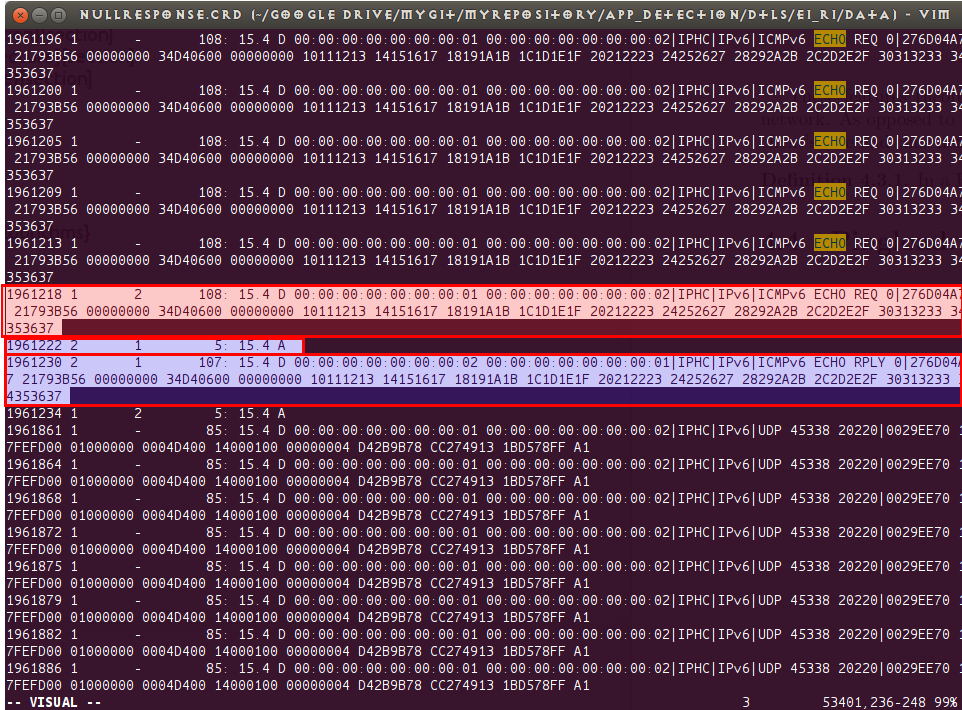
\includegraphics[width=\textwidth,]{fig/responsetime.png}
}
\caption{Capture of a ping packet}
\label{fig: ping packet}
\end{figure}

\begin{table}[!]
\centering
\begin{tabular}{|l|l|l|l|l|}
\hline
Time (ms) & From (ID) & To (ID) & Length (bytes) & Type          \\ \hline
1961218   & 1         & 2       & 108            & ICMP ECHO \\ \hline
1961222   & 2         & 1       & 5              & 802.15.4 ACK  \\ \hline
1961230   & 2         & 1       & 107            & ICMP ECHO \\ \hline
\end{tabular}
\caption{Packet Features of an ICMP ECHO request and response}
\label{Tbl: ping}
\end{table}

Three packets are marked out in \Cref{fig: ping packet} which forms an instance of ICMP ECHO\cite{rfc1122} (also known as PING) session. The extracted packet features are displayed in \Cref{Tbl: ping}.

\begin{description}
\item[Explanation of the Packets:]\hfill \\
The first packet is an ICMP ECHO request and the third packet being its response. The second packet is a 802.15.4 ACK\footnote{This is an acknowledgement from the receiver that notifies the sender that the packet has been received.} and is thus transparent to the upper ICMP protocol.
\end{description}

From this example we can see that the RI for this PING session is:
\begin{equation*}
1961230 - 1961218 = 12 \text{(ms)}
\end{equation*}

\end{example}

Timing information can be exploited by several attacks, such as \cite{Peekaboo} and \cite{rsatiming}.

We have experimentally measured a RNG\footnote{Random Number Generator} call on Wismote platform in the Cooja simulator is roughly 0.3 ms.

\section{PINGLOAD: PING side-channel for Payload }
Support of ICMP ECHO is required by \cite{rfc1122} and is also enabled in Contiki OS by default. However, our experimental results shows that the response time of these ping packets could potentially be exploited to reveal the application running on target sensor node.

We call such technique {\bf  Application Fingerprinting}.

\subsection{Hypothesis}
A phenomenon we realised is that when a ping packet arrived while the target node is executing some payload, say reading a sensor or processing data, the PING RI begins to vary comparing to a stable value  when no there is no payload. 

\begin{example}
\begin{figure}
\centering
{
  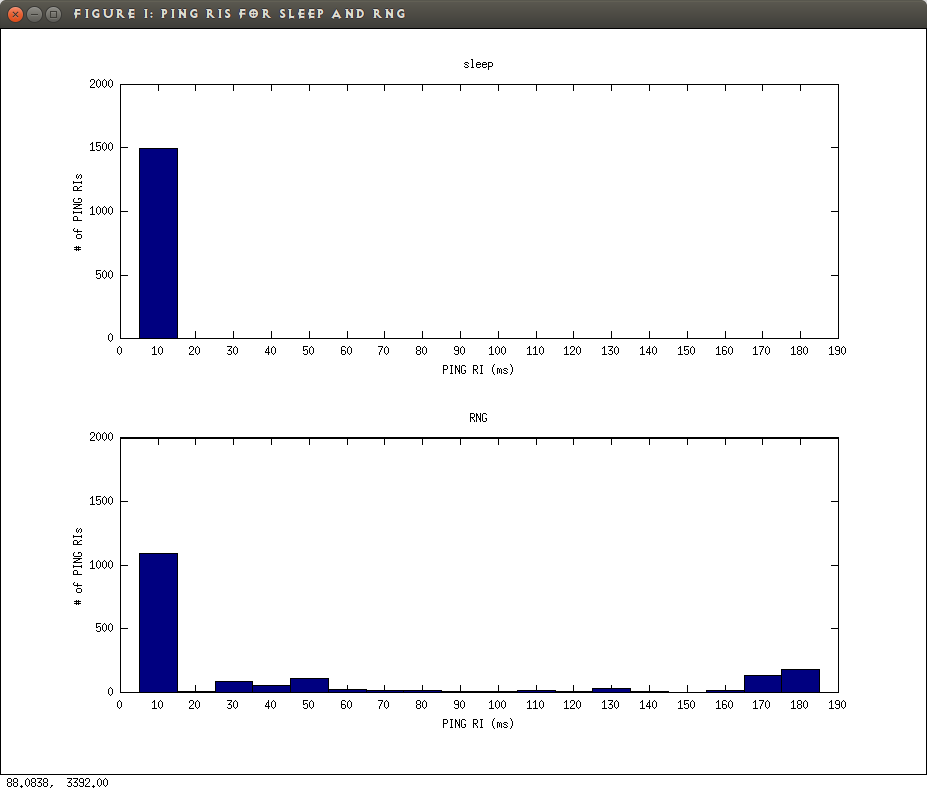
\includegraphics[width=1\textwidth]{fig/pingri.png}
}
\caption{An example of PING RIs with different payload}
\label{Fig: PINGLOAD RIs}
\end{figure}
\Cref{Fig: PINGLOAD RIs} shows RIs of PING collected in two experiments. The upper half are collected with the target is constantly sleep whilst the lower half occasionally receives a request which triggers the target to call RNG. We can see that the PING RI varies alongside the target is given some payload from this figure.
\end{example}

The data shown in \Cref{Fig: PINGLOAD RIs} suggests that the “plain”, that is without any interference, PING RI is 12 to 13 ms. Further more, those variations of  PING RI is very likely caused by the payload of the target.

This experiment inspired that the distributions of PING RIs might vary according to the payload of target and could possibly considered as an fingerprint of the target’s application. In other word, an adversary could possibly tell whether the target is running a specific application by looking at its PING RIs distribution.

The attack is strait forward:
\begin{description}
\item[Profile sleep RIs]: \hfill\\
The PING RIs for a sleeping node of the same platform can be profiled by pinging a sleeping node. We denote the sleeping profile as $RI_{sleep}$. 

\item[Fingerprint application]: \hfill\\
The adversary collects PING RIs on a profiling node with known application. The profiling node needs to be of the same platform and executing the same code of the target’s. The application fingerprint denotes as: $F_p=\{p_1, p_2, ... , p_n\}$. 

\item[Collect fingerprint of target]: \hfill\\
The adversary then collects the PING RI for the target node by pinging it. We denote the collected data as: $F_t=\{t_1, t_2, ..., t_m\}$.

\item[Extract Featured RIs]: We can remove them from the data sets and keep the PING RIs those has been interfered by the application. We denote the extracted RIs as \textbf{Featured RIs}:
\begin{eqnarray*}
F’_p = \{x | x \in F_p,  x \notin RI_{sleep}\}\\
F’_p = \{x | x \in F_t,  x \notin RI_{sleep}\}
\end{eqnarray*}

Practically speaking, the PING protocol are designed to be responded immediately for diagnosis purpose; hence $RI_{sleep}$ usually has an extremely low variance and its mean is also much less than $F_p$ and $F_t$.

Using the Featured RIs not only provides a better vision of the fingerprint but also removes the error caused by different frequency of the target code being executed, as all the Featured RIs are actually collected when the node is at a non-sleeping state. 

\item[Estimate Distribution (Optional)]: \hfill\\
We then estimate the distributions of $F’_p$ and $F’_t$, denote as $D_p$ and $D_t$. A naive method is to simply use their histograms. An example of such histograms are shown as \Cref{Fig: featuredri_rng}.

\begin{figure}
\center
{
	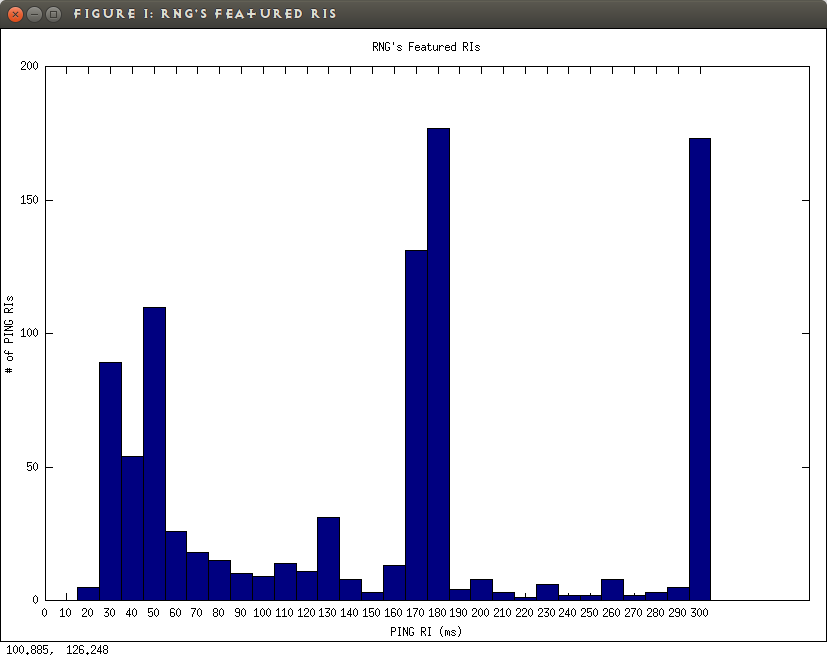
\includegraphics[width=0.49 \textwidth]{fig/featuredri_rng1.png}
	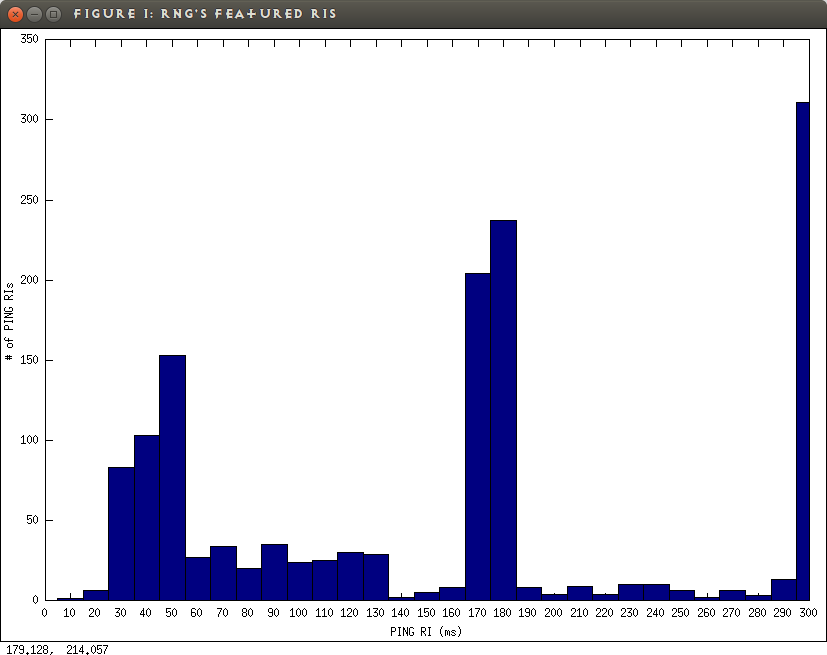
\includegraphics[width=0.49 \textwidth]{fig/featuredri_rng2.png}
}
\caption{Two examples of RNG’s Featured RIs histogram}
\label{Fig: featuredri_rng}
\end{figure}

\item[Distinguish Distributions]: \hfill\\
Finally we test whether $D_t$ and $D_p$ are the same distribution. An naive way is to compute the correlation of counts of the histograms. We conclude the target node is running the profiled application if $D_t$ and $D_p$ are the same distribution.
\end{description}

Practically speaking, the key point of Application Fingerprinting is to test whether the target’s Featured RIs, i.e. $F’_t$, is sampled from same distribution of the profiled one, i.e. $F’_p$; therefore estimating their distribution might not be necessary for some statistical methods such as t-tests. However as we can see in \Cref{Fig: featuredri_rng}, PING RIs’ distribution are very unlikely to be normalised. Therefore a future work is to find a better distinguishing method than the current naive one.

\subsection{Experiment Result}
We tried our Application Fingerprinting method above on a Cooja simulated Wismote platform with different code. \textbf{In conclusion, the fingerprint appears to be effective for certain circumstances but will tends to result into false positives as the profiled application and target application gets similar to each other.}

To be more specifically, the target node execute some specific code upon receiving an application layer protocol request, similar to CoAP. Further more, all traffic are protected by DTLS with TLS\_PSK\_WITH\_AES\_128\_CCM\_8 ciphersuite. Both intervals of PINGs and the application request are set to some asynchronised value to avoid overflooding the target and to create a ‘more realistic’ simulation.

Everything other than the examined code are the same for all experiments. Two samples are collected independently for each code to simulate a fingerprinting scenario. The histograms are clustered by 5ms.

We examined two classes of codes:
\begin{description}
\item[RNG Calls]: \hfill\\
The target node repeatedly calls RNG for $i$ times. We examined their Featured PING RI for different values of $i$. The reason for picking RNG is that on some platforms where a hardware RNG is provided, the call to it is expected to be similar to a call to a sensor reading which is actually an interrupt. Results are shown in \Cref{Tbl: pingload RNG}.

\item[Arithmetic Operations]: \hfill\\
The target node repeatedly does arithmetic operations, namely addition, multiplication and modular, on two random generated word size integers for 10000 times. This class is particularly interested from a cryptographic point of view as the number of arithmetic operations could potentially developed to key recovering attacks. Results are shown in \Cref{Tbl: pingload arth}.
\end{description}



\begin{table}
\centering
\begin{tabular}{|c|cccc}
\hline
\textit{\textbf{Correlations}} & \multicolumn{1}{c|}{i=50} & \multicolumn{1}{c|}{i=100} & \multicolumn{1}{c|}{i=2500} & \multicolumn{1}{c|}{i=5000} \\ \hline
i=50                           & \textbf{0.988}            & 0.891                      & -0.014                      & -0.033                      \\ \cline{1-1}
i=100                          & 0.891                     & \textbf{0.973}             & -0.025                      & -0.042                      \\ \cline{1-1}
i=2500                         & -0.014                    & -0.025                     & \textbf{0.993}              & -0.035                      \\ \cline{1-1}
i=5000                         & -0.033                    & -0.042                     & -0.035                      & \textbf{0.985}              \\ \cline{1-1}
\end{tabular}
\caption{Correlations for RNG}
\label{Tbl: pingload RNG}
\end{table}

\begin{table}
\centering
\begin{tabular}{|c|ccc}
\hline
\textit{\textbf{Correlations}} & \multicolumn{1}{c|}{+} & \multicolumn{1}{c|}{*} & \multicolumn{1}{c|}{\%} \\ \hline
+                              & \textbf{0.990}         & \textbf{0.990}         & \textbf{0.988}          \\ \cline{1-1}
*                              & \textbf{0.990}         & \textbf{0.989}         & \textbf{0.985}          \\ \cline{1-1}
\%                             & \textbf{0.988}         & \textbf{0.985}         & \textbf{0.984}          \\ \cline{1-1}
\end{tabular}
\caption{Correlations for word arithmetic operations}
\label{Tbl: pingload arth}
\end{table}

\begin{table}[]
\centering
\begin{tabular}{|c|c|}
\hline
\textbf{\textit {Correlations}} & +     \\ \hline
i=50         & 0.877 \\ \hline
\end{tabular}
\caption{Correlation for $i=50$ and addition}
\label{Tbl: pingload rng arth}
\end{table}

We also computed the correlation for $i=50$ and addition, as shown in \Cref{Tbl: pingload rng arth}.

The results suggests the following conjectures:
\begin{enumerate}
\item The results for RNG suggests that the fingerprinting is effective for this class of code, as the same code results into nearly perfect correlations ($\geq 0.95$).

\item Even relatively slight changes can be detected, as we can see the correlation dropped to $0.891$ alongside 50 iterations of RNG calls (50 RNG calls take about 1.4ms).

\item The results for arithmetic operations indicates that their  fingerprint are unlikely to be distinguishable. There are two potential causes we have considered:
\begin{enumerate}
\item The differences between these operations are too small to be detected.

\item Experiment methodology error. Since the target node we used during the experiments call RNG twice upon each request to generate two operands whilst the word arithmetic operations have much lighter weigh comparing to RNG at magnitude level; thus the fingerprint is dominated by RNG rather than word arithmetic operations. As a result, we can see that a relatively high correlation can be observed between word addition and 50 RNG calls as shown in \Cref{Tbl: pingload rng arth}.
\end{enumerate}
\end{enumerate}

\subsection{General Hypothetical Model}
THE BLACK BOX MODEL
\chapter{Fulture Work}

Use Kolmogorov-Smirnov test to compare PING RIs.
\appendix
\chapter{OrderFlavour-Length leakage channel}
\label{OrderFlavour leakage channel}

In this application, the joint probability of $Order$ and $Flavour$ are simply the product of their marginal probability. However, since “ESPRESSO” will always followed by $Flavour$ of of both degree of SUGAR and MILK being $0$(see  \Cref{ESPRESSO}); hence
\begin{eqnarray*}
P(x_1, x_2 | \text{“ESPRESSO”}) = 
	\begin{cases}
	1 &\text{if } x_1 = x_2 = 0\\
	0 &\text{otherwise}
	\end{cases}
\end{eqnarray*}

Therefore
\begin{eqnarray*}
P(\text{“ESPRESSO”}, x_1, x_2 ) = 
	\begin{cases}
	1/4 &\text{if } x_1 = x_2 = 0\\
	0 &\text{otherwise}
	\end{cases}
\end{eqnarray*}


%\bibliographystyle{ieeetran}
%\bibliography{references,rfc}
\printbibliography

\end{document}
